
\section{Performance Evaluation}

We implemented the rotation-invariant convolution using four different approaches: (1) our scatter based kernel, (2) a cuDNN based pipeline, (3) an Oriented Response Networks (ORN) implementation, and (4) an equivariant convolution implementation using the e2cnn library. 

In our scatter based approach, the four symmetric rotations are processed within a single fused convolution, so each input element is multiplied only once.
In contrast, the cuDNN based pipeline must treat every rotated filter as an independent kernel, performing four separate convolution and therefore four distinct multiply–accumulate passes before the results can be combined. 
The ORN and e2cnn implementations follow their respective rotation-equivariant formulations and are included as additional baselines for comparison.
Among these, we implemented the backward pass for the scatter-based and cuDNN-based versions, as automatic gradient computation is not available for these custom rotation-invariant operations, ensuring that gradients propagate correctly through every rotated filter.

\subsection{Model for Evaluation}\label{subsubsec:model}
To evaluate the performance of the scatter based rotation invariant convolution in a real segmentation application, we replaced the first convolution of base convolution block in UNet \cite{ronneberger2015u} with the rotation invariant convolution described above (see Fig. \ref{fig:unet} for illustration). To balance performance and dimension explosion, we apply max pooling across every four symmetric rotations; for example, with eight rotations, this produces two orientation features, each corresponding to a group of four symmetric rotations. The second convolution within the base block uses a standard convolution, we found through experiments that this design improves performance.
\begin{figure}[h]
    \centering
    \begin{subfigure}[b]{0.49\textwidth}  % 49% to avoid overflow
        \centering
        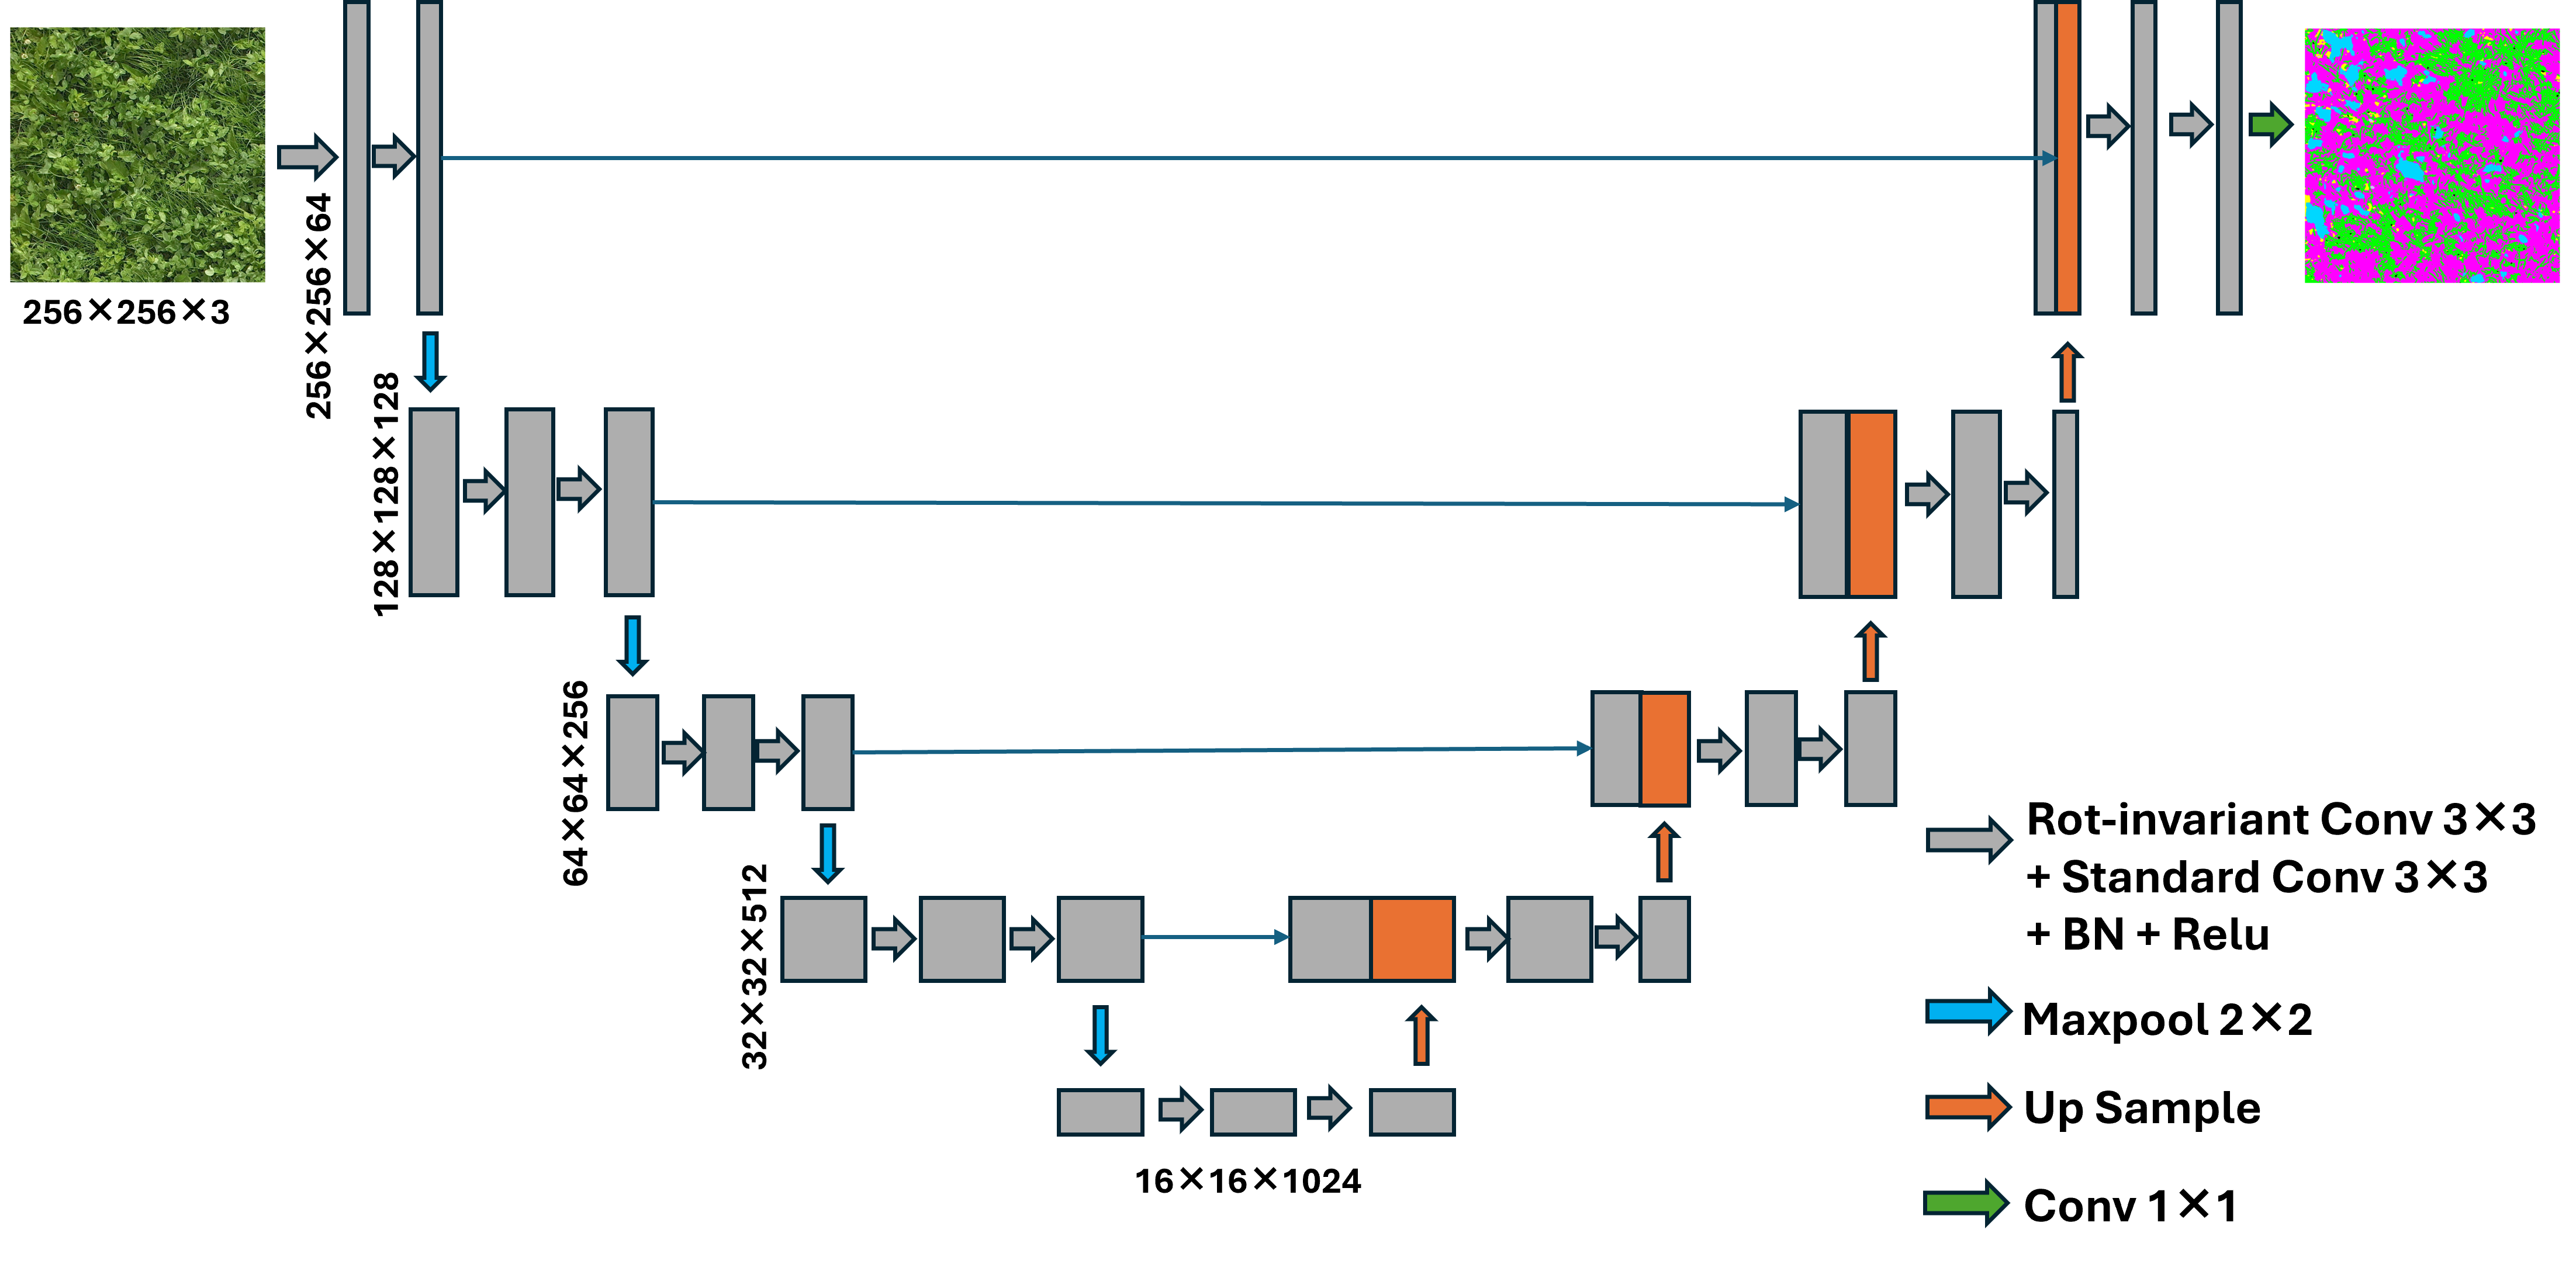
\includegraphics[width=\textwidth]{fig/unet/unet.png}
    \end{subfigure}
    \caption{Unet architecture with rotation invariant convolution block.}
	\vspace{-0.4cm}
    \label{fig:unet}
\end{figure}


\subsection{Datasets for Training and Testing}\label{subsec:dataset}
The modified UNet were trained and tested on two datasets: an in-farm plant-segmentation dataset captured with a DJI M300 drone \cite{dji_m300} equipped with a P1 photogrammetry camera \cite{dji_p1}, and the public Semantic Segmentation Drone Dataset \cite{semantic_drone_dataset}. All experiments were conducted on an Ubuntu 22.04 system equipped with eight NVIDIA RTX 3090 GPUs.

\subsubsection{Plant segmentation dataset}\label{subsubsec:plant}
Accurately measuring species composition in pasture and forage systems is fundamental for biodiversity monitoring and precision agriculture because it informs management decisions on seeding, fertilization, and grazing intensity. However, mixed‑species pastures are highly heterogeneous: the realized stand rarely matches the seed plan and can vary widely across a field and over time. This variability places stringent demands on automated, high‑resolution, plant‑level segmentation of aerial/UAV imagery. Because leaves and other canopy structures appear at arbitrary orientations in overhead views, incorporating rotation invariance into the segmentation pipeline is critical for robust species discrimination in multi‑species pastures.

We mapped pasture species composition from high‑resolution UAV imagery acquired with a DJI drone equipped with a Zenmuse P1 camera. Flights were conducted at approximately 12 m above ground level,
yielding a nominal ground sampling distance (GSD) of {0.15} cm per pixel.
Forward image overlap was 80\%,
and each P1 frame covered roughly {12.31 x 8.20} m$^2$ on the ground.
This dataset contains 1000 samples and we use 800 samples for training and 100 for validation and 100 for test.

\subsubsection{Semantic Segmentation Drone dataset}\label{subsec:droneDataset}
The Semantic Drone Segmentation dataset contains 400 high-resolution nadir-view images of urban residential scenes, captured at altitudes between 5 m and 30 m above ground and annotated with detailed pixel-level semantic labels covering 24 object categories. In our experiments, we use 340 images for training, 32 for validation, and 28 for testing.



\subsection{Evaluation with Different Convolution Approaches}\label{subsubsec:differentConvs}

\subsubsection{Single orientation rotation convolution}\label{subsubsec:singleOri}
Given that single-orientation rotation convolution collapses to standard convolution, we first conduct a direct comparison between our scatter-based convolution API and cuDNN’s standard convolution API. The corresponding results are reported in Appendix~\ref{appendix:compareCUDNN}.

We compare our approach with cuDNN as well as the state-of-the-art ORN \cite{orn} and E2CNN \cite{e2cnn} frameworks, both of which provide APIs for achieving rotation invariance.
Tables \ref{tab:single-plant} and \ref{tab:single-drone} report the performance of cuDNN, ORN, E2CNN, and the proposed scatter-based convolution under the single-orientation setting.
The observed accuracy variation is within $\pm 0.1\%$.
Since single-orientation rotation convolution degenerates to standard convolution, all methods achieve nearly identical segmentation accuracy. Nevertheless, notable differences arise in computational efficiency.
On the plant dataset with 256×256 inputs, E2CNN achieves the lowest training time and energy consumption, while scatter-based convolution also demonstrates competitive efficiency, training approximately 9.2\% faster than cuDNN and reducing energy consumption by about 6.9\%. At 1024×1024 resolution, scatter-based convolution achieves the best efficiency, reducing training time by roughly 7.0\% and energy usage by 7.6\% compared with cuDNN.
Similar trends are observed on the drone dataset: at 256 resolution, E2CNN attains the highest accuracy and lowest computational cost, whereas scatter-based convolution remains consistently more efficient than cuDNN. At 1024 resolution, scatter-based convolution outperforms all baselines in both training time (7.1\% reduction) and energy consumption (7.9\% reduction).
These results indicate that while E2CNN is particularly efficient for smaller input resolutions, the proposed scatter-based convolution provides consistent and scalable efficiency gains—especially at higher resolutions—without sacrificing segmentation accuracy, as it avoids explicit data lowering and reduces memory traffic through direct scatter accumulation.
Representative segmentation results are visulized in Fig. \ref{fig:plant} and Fig. \ref{fig:drone}.

%We compare our approach with cuDNN as well as the state-of-the-art ORN \cite{orn} and E2CNN \cite{e2cnn} frameworks, both of which provide APIs for achieving rotation invariance.
%Tables \ref{tab:single-plant} and \ref{tab:single-drone} present the performance of cuDNN, ORN, E2CNN, and our scatter-based convolution under the single-orientation setting. Because single-orientation rotation convolution degenerates to standard convolution, all methods achieve nearly identical accuracy. Nevertheless, meaningful differences appear in computational cost. On the plant dataset with 256×256 inputs, scatter-based convolution trains approximately 9.2\% faster than cuDNN and reduces energy consumption by about 6.9\%. At 1024×1024 resolution, scatter achieves roughly a 7.0\% reduction in training time and a 7.6\% reduction in energy usage. Similar trends are seen on the drone dataset, where scatter-based convolution is about 9.8\% faster at 256 resolution and 7.1\% faster at 1024 resolution, while saving approximately 5.9\% and 7.9\% energy, respectively. These results show that even in the absence of multi-orientation modeling, the scatter based convolution offers consistent efficiency gains without sacrificing accuracy. Fig. \ref{fig:plant} and Fig. \ref{fig:drone} show representative segmentation predictions for plant dataset and drone view datasets.

\begin{table}[ht]
\centering
\caption{Plant Data Segmentation Using Various Single-Orientation Rotation-Invariant Convolutions}
\renewcommand{\arraystretch}{1.2}
\begin{tabular}{c|c|c|c|c} 
\hline\hline
\shortstack{Image\\size} & 
\shortstack{Convolution\\applied} & 
\shortstack{Training\\time (s)} &  
\shortstack{Energy\\(kWh)} &  
\shortstack{Test\\accuracy (\%)} \\ 
\hline\hline
\multirow{4}{*}{256} 
 & cudnn based conv    & 8604.0  & 0.379  &73.59  \\ \cline{2-5}
 & ORN conv            & 7758.0  & 0.362  &73.63  \\ \cline{2-5}
 & E2CNN conv          & 7116.0  & 0.315  & 73.73 \\ \cline{2-5}
 & scatter based conv  & 7808.0  & 0.353  &73.62  \\
\hline

\multirow{4}{*}{1024} 
 & cudnn based conv    & 26153.0 & 1.758  &71.32  \\ \cline{2-5}
 & ORN conv            & 25538.0 & 1.719  &71.38  \\ \cline{2-5}
 & E2CNN conv          & 27405.0 & 2.213  &71.66  \\ \cline{2-5}
 & scatter based conv  & 24317.0 & 1.625  &71.28  \\
\hline
\end{tabular}
\label{tab:single-plant}
\end{table}

\begin{figure}[htbp]
  \centering

  %------------- top -------------
  \begin{subfigure}{0.45\textwidth}
    \centering
    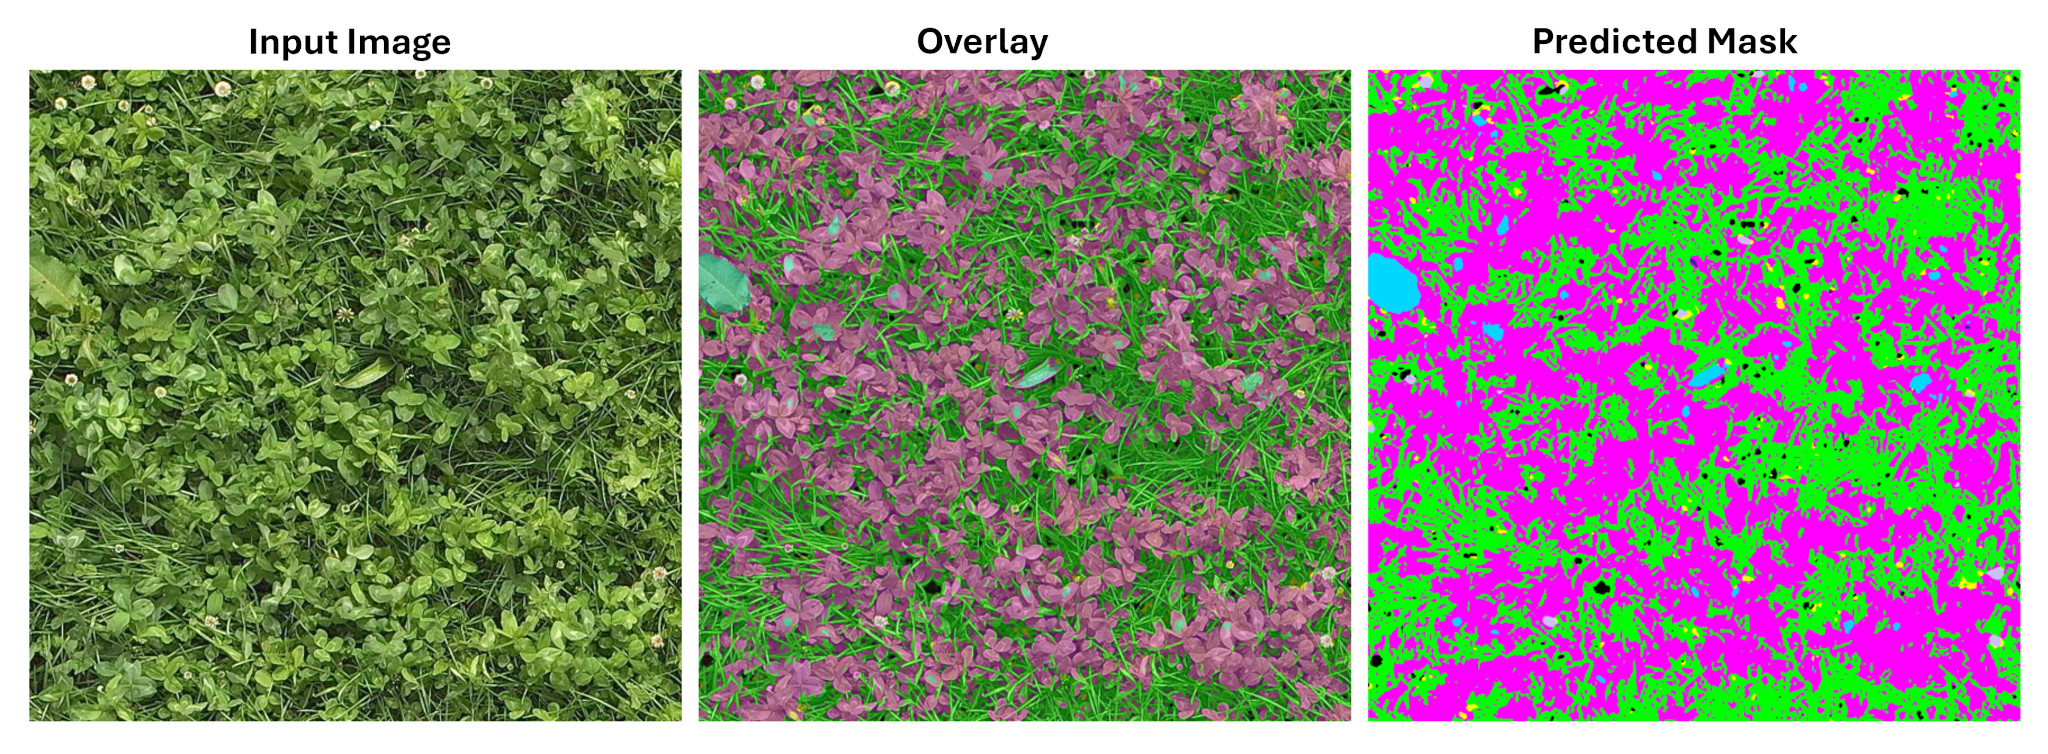
\includegraphics[width=\textwidth]{fig/FL_timing/infer-img-grass/seg-1.jpg}
  \end{subfigure}
  \par\vspace{0.3em}

  %----------- middle ------------
  \begin{subfigure}{0.45\textwidth}
    \centering
    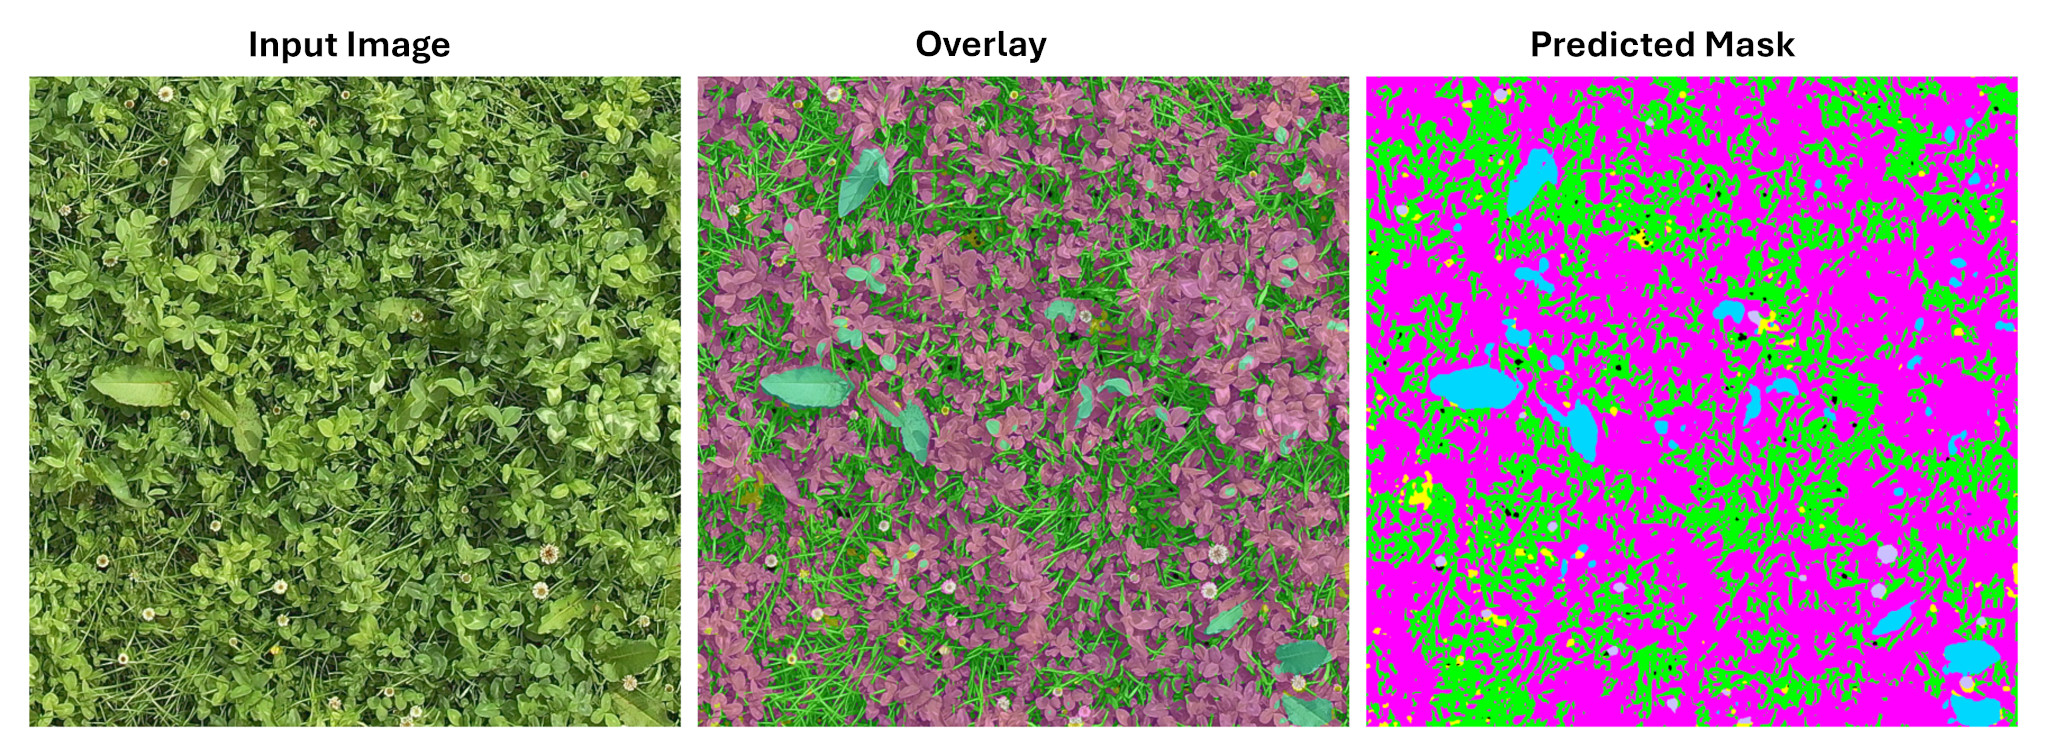
\includegraphics[width=\textwidth]{fig/FL_timing/infer-img-grass/seg-2.jpg}
  \end{subfigure}
  \par\vspace{0.3em}

  %----------- bottom ------------
  \begin{subfigure}{0.45\textwidth}
    \centering
    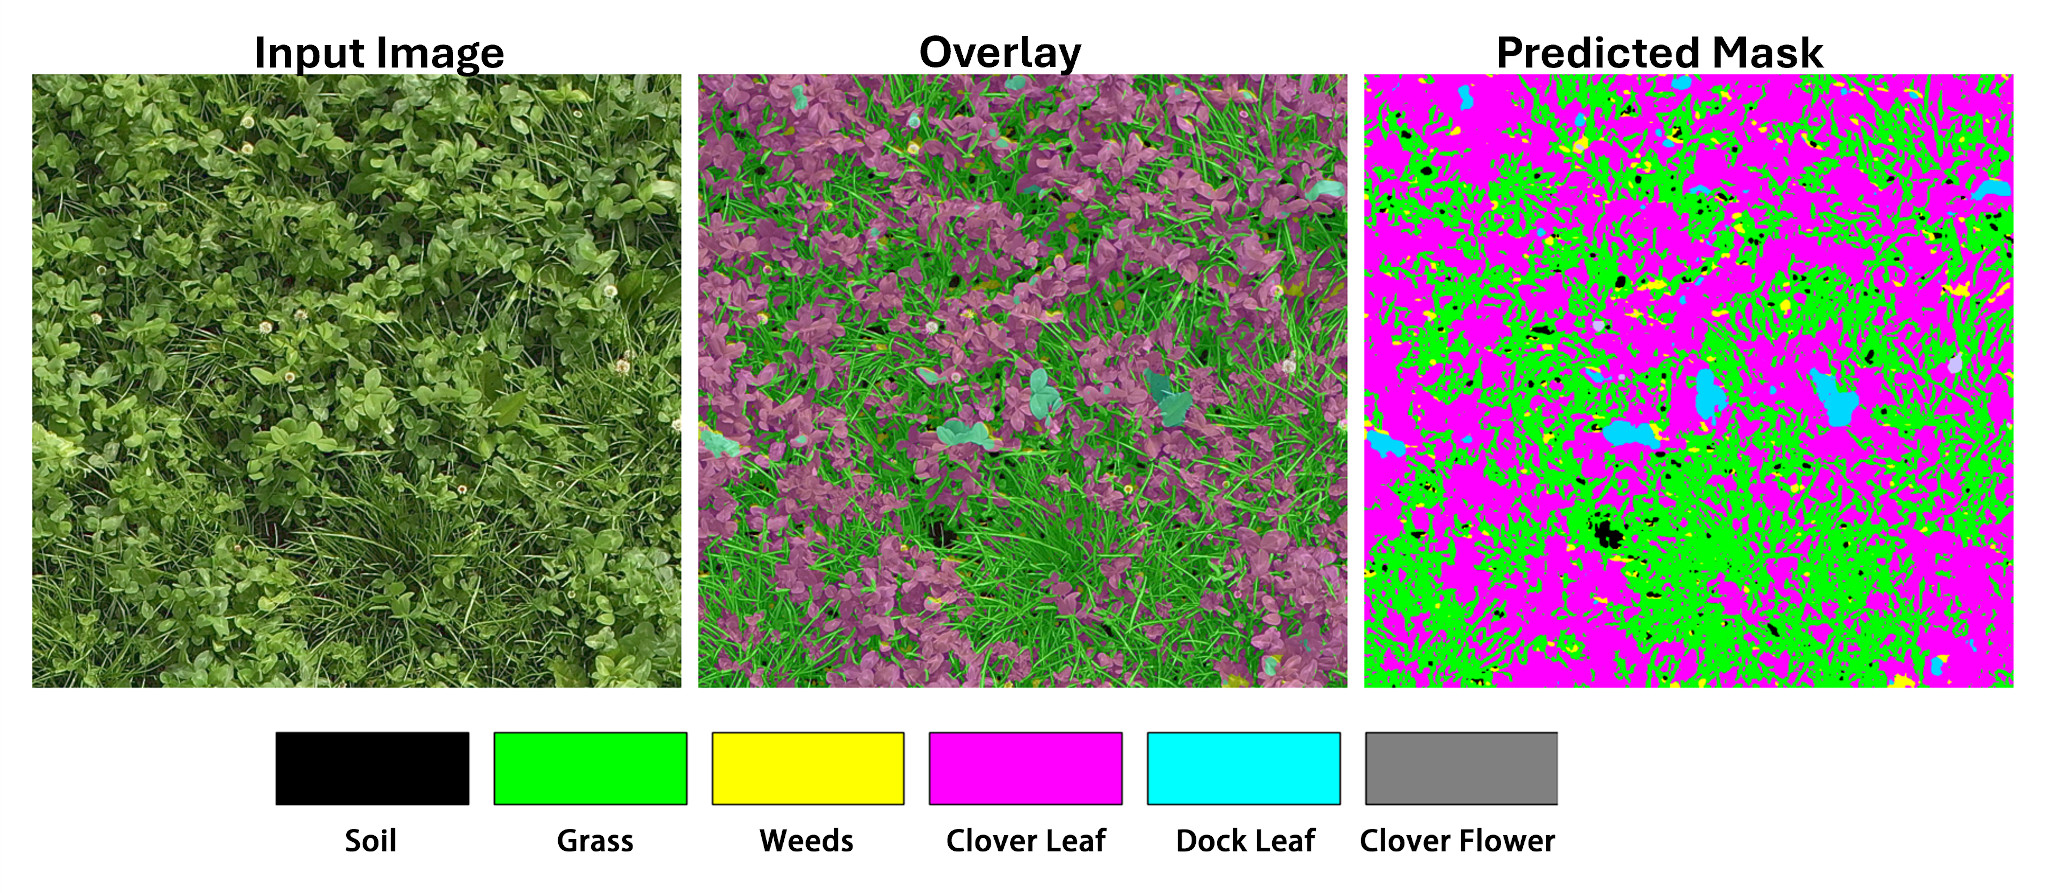
\includegraphics[width=\textwidth]{fig/FL_timing/infer-img-grass/seg-3.jpg}
  \end{subfigure}

  \caption{Visualization of segmentation results on plant data.}
  \label{fig:plant}
\end{figure}


\begin{table}[ht]
\centering
\caption{Semantic drone segmentation Using Various Single-Orientation Rotation-Invariant Convolutions}
\renewcommand{\arraystretch}{1.2}
\begin{tabular}{c|c|c|c|c} 
\hline\hline
\shortstack{Image\\size} & 
\shortstack{Convolution\\applied} & 
\shortstack{Training\\time (s)} &  
\shortstack{Energy\\(kWh)} &  
\shortstack{Test\\accuracy (\%)} \\ 
\hline\hline
\multirow{4}{*}{256} 
 & cudnn based conv    & 3242.2  & 0.1408 &90.62  \\ \cline{2-5}
 & ORN conv    & 2945.1 & 0.1359  &90.67  \\ \cline{2-5}
 & E2CNN conv    &2705.7 &0.1186  &90.73  \\ \cline{2-5}
 & scatter based conv  & 2925.6  & 0.1325 &90.65  \\
\hline

\multirow{4}{*}{1024} 
  & cudnn based conv   & 9865.5  &0.6618 &88.71  \\ \cline{2-5}
 & ORN conv    &9726.3  &0.6498  &88.74  \\ \cline{2-5}
 & E2CNN conv    &10392.7 & 0.8372  & 88.78 \\ \cline{2-5}
 & scatter based conv  &9166.9  & 0.6094&88.69  \\
\hline
\end{tabular}
\label{tab:single-drone}
\end{table}


\begin{figure}[htbp]
  \centering
  
  %------------- top -------------
  \begin{subfigure}{0.45\textwidth}
    \centering
    
\includegraphics[width=\textwidth]{fig/FL\_timing/infer-img-drone/drone-seg-1.jpg}
   
    %\label{fig:a}
  \end{subfigure}\par\medskip
  
  %----------- middle ------------
  \begin{subfigure}{0.45\textwidth}
    \centering
    
\includegraphics[width=\textwidth]{fig/FL\_timing/infer-img-drone/drone-seg-2.jpg}
  
   % \label{fig:b}
  \end{subfigure}\par\medskip
  
  %----------- bottom ------------
  \begin{subfigure}{0.44\textwidth}
    \centering
    
\includegraphics[width=\textwidth]{fig/FL\_timing/infer-img-drone/drone-seg-3.jpg}
  
  %  \label{fig:c}
  \end{subfigure}

  \caption{Visualization of segmentation results on Semantic Segmentation Drone dataset.}
  \label{fig:drone}
\end{figure}


\subsubsection{Symetric four orientation rotation convolution}\label{subsubsec:fourOri}
%Tables \ref{tab:four-plant} and \ref{tab:four-drone} summarize the results for the symmetric four-orientation configuration. Relative to single-orientation convolution, accuracy improves slightly, particularly for E2CNN, reflecting the benefit of limited rotation modeling. The computational advantages of scatter-based convolution become more pronounced under this setting. On the plant dataset, scatter reduces training time by approximately 45.8\% at 256 resolution and 28.8\% at 1024 resolution, while lowering energy consumption by about 38.4\% and 18.5\%, respectively. On the drone dataset, scatter provides comparable benefits, achieving about 46.7\% faster training at 256 resolution and 32.9\% at 1024 resolution, with corresponding energy reductions of roughly 39.1\% and 22.8\%. These results indicate that symmetric four-orientation convolutions provide a strong balance between improved segmentation accuracy and computational efficiency, with scatter based convolution offering the best performance–efficiency trade-off.

Tables \ref{tab:four-plant} and \ref{tab:four-drone} summarize the results for the symmetric four-orientation configuration. Relative to single-orientation convolution, accuracy increases by about 2\%, with E2CNN achieving the highest accuracy, reflecting the benefit of four rotation modeling. The computational advantages of scatter-based convolution become more pronounced under this setting. On the plant dataset, scatter reduces training time by approximately 45.9\% at 256 resolution and 28.8\% at 1024 resolution, while lowering energy consumption by about 38.4\% and 18.6\%, respectively. On the drone dataset, scatter provides comparable benefits, achieving about 46.7\% faster training at 256 resolution and 32.9\% at 1024 resolution, with corresponding energy reductions of roughly 39.1\% and 22.8\%. These results indicate that symmetric four-orientation convolutions achieve strong segmentation accuracy with manageable computational cost. The scatter based convolution provides the most favorable accuracy–efficiency profile, benefiting from reuse of intermediate computations across symmetric rotations. This enables substantial reductions in training time and energy consumption while maintaining segmentation accuracy.

\begin{table}[ht]
\centering
\caption{Plant Data Segmentation Using Various Four-Orientation Rotation-Invariant Convolutions}
\renewcommand{\arraystretch}{1.2}
\begin{tabular}{c|c|c|c|c} 
\hline\hline
\shortstack{Image\\size} & 
\shortstack{Convolution\\applied} & 
\shortstack{Training\\time (s)} &  
\shortstack{Energy\\(kWh)} &  
\shortstack{Test\\accuracy (\%)} \\ 
\hline\hline
\multirow{4}{*}{256} 
 & cudnn based conv    & 20234.6  & 0.943  &75.64  \\ \cline{2-5}
 & ORN conv            & 20154.2  & 0.921  &  75.69\\ \cline{2-5}
 & E2CNN conv          & 18575.8  & 0.783  & 75.71 \\ \cline{2-5}
 & scatter based conv  & 10962.6  & 0.581  & 75.61 \\
\hline
\multirow{4}{*}{1024} 
 & cudnn based conv    & 82081.0  & 5.564   &72.92  \\ \cline{2-5}
 & ORN conv            & 81706.5  & 5.623   &72.98  \\ \cline{2-5}
 & E2CNN conv          & 76175.0  & 5.118   &73.05  \\ \cline{2-5}
 & scatter based conv  & 58433.9  & 4.532   &72.95  \\
\hline
\end{tabular}
\label{tab:four-plant}
\end{table}

\begin{table}[ht]
\centering
\caption{Semantic drone segmentation Using Various Four-Orientation Rotation-Invariant Convolutions}
\renewcommand{\arraystretch}{1.2}
\begin{tabular}{c|c|c|c|c} 
\hline\hline
\shortstack{Image\\size} & 
\shortstack{Convolution\\applied} & 
\shortstack{Training\\time (s)} &  
\shortstack{Energy\\(kWh)} &  
\shortstack{Test\\accuracy (\%)} \\ 
\hline\hline
\multirow{4}{*}{256} 
 & cudnn based conv    &7713.1  &0.3570 &91.88  \\ \cline{2-5}
 & ORN conv    &7651.6  &0.3501  &91.93  \\ \cline{2-5}
 & E2CNN conv    &6908.2 &0.2943  &92.06  \\ \cline{2-5}
 & scatter based conv  &4109.6  &0.2175 &91.88  \\
\hline
\multirow{4}{*}{1024} 
  & cudnn based conv    &30936.5  &2.103 &90.39  \\ \cline{2-5}
 & ORN conv    &31025.2  & 2.203  &90.41  \\ \cline{2-5}
 & E2CNN conv    &28925.6 &1.946  &90.62  \\ \cline{2-5}
 & scatter based conv  &20761.8  & 1.623&90.43  \\
\hline
\end{tabular}
\label{tab:four-drone}
\end{table}

\subsubsection{Symetric eight orientation rotation convolution}\label{subsubsec:eightOri}
%Tables \ref{tab:eight-plant} and \ref{tab:eight-drone} report the eight-orientation results. Increasing the number of modeled orientations leads to further accuracy improvements, especially for the plant dataset. Because convolutional pooling over eight orientations produces twice the feature-map dimensionality of the four-orientation configuration, it imposes substantially greater memory and computational demands on conventional implementations.The scatter-based convolution continues to provide substantial efficiency benefits. On the plant dataset, scatter is approximately 45.4\% faster than cuDNN at 256 resolution and about 20.8\% faster at 1024 resolution, while reducing energy usage by approximately 41.2\% and 12.9\%, respectively. On the drone dataset, scatter achieves around 56.9\% faster training at 256 resolution and 32.9\% at 1024 resolution, with energy savings of about 44.3\% and 22.8\%. These comparisons show that as rotation resolution increases, rotation-invariant convolutions become more accurate, and the scatter-based implementation remains significantly more efficient than ORN and E2CNN, consistently delivering between 20\% and 55\% faster training and 15\% to 45\% lower energy consumption. ORN shows lower accuracy improvements in the eight-orientation setting because it does not provide an API for orientation-subgroup pooling; instead, it produces a single pooled feature over all eight orientations. 
 
Tables \ref{tab:eight-plant} and \ref{tab:eight-drone} report the eight-orientation results. Increasing the number of modeled orientations leads to further accuracy improvements, especially for the plant dataset. Because convolutional pooling over eight orientations produces twice the feature-map dimensionality of the four-orientation configuration. However, it imposes substantially greater memory and computational demands on conventional implementations. The scatter based convolution continues to provide substantial efficiency benefits.
On the plant dataset, scatter is approximately 45.4\% faster than cuDNN at 256 resolution and about 34.5\% faster at 1024 resolution, while reducing energy usage by approximately 41.2\% and 21.7\%, respectively.
On the drone dataset, scatter achieves around 56.9\% faster training at 256 resolution and 32.7\% faster at 1024 resolution, with energy savings of about 44.3\% and 22.7\%, respectively.

The proposed scatter-based approach differs from E2CNN in how rotation is modeled. While E2CNN learns orientation-dependent expansion coefficients, the scatter-based method constructs steerable filters from a set of learnable base filters, as described in Section~\ref{sec:fft_arbitrary}, where orientation dependence is introduced analytically. By enforcing orthogonality and equal-magnitude constraints on these base filters, the formulation approximates rotation invariance, leading to accuracy trends distinct from E2CNN.

The experimental results demonstrate that as rotation resolution increases, rotation invariant convolutions become more accurate, and the scatter based implementation remains more efficient than ORN and E2CNN. ORN shows smaller accuracy improvements in the eight-orientation setting because it does not provide an API for orientation-subgroup pooling; in our implementation, its group pooling operation aggregates all eight orientations into a single pooled feature.
As accuracy continues to improve, conventional rotation-invariant convolutions incur rapidly increasing memory and computation overhead due to expanded feature-map dimensionality.
This effect is particularly evident for E2CNN, where group representations lead to larger intermediate tensors.
By contrast, the proposed scatter-based implementation mitigates this issue by consolidating rotation handling within a single convolution pass, thereby maintaining scalability as orientation resolution increases.

\begin{table}[ht]
\centering
\caption{Plant Data Segmentation Using Various Eight-Orientation Rotation-Invariant Convolutions}
\renewcommand{\arraystretch}{1.2}
\begin{tabular}{c|c|c|c|c} 
\hline\hline
\shortstack{Image\\size} & 
\shortstack{Convolution\\applied} & 
\shortstack{Training\\time (s)} &  
\shortstack{Energy\\(kWh)} &  
\shortstack{Test\\accuracy (\%)} \\ 
\hline
\hline
\multirow{4}{*}{256} 
 & cudnn based conv    & 36866.0  & 1.675  & 78.69 \\ \cline{2-5}
 & ORN conv            & 36188.0  & 1.612  & 76.13 \\ \cline{2-5}
 & E2CNN conv          & 33408.0  & 1.561  &78.15  \\ \cline{2-5}
 & scatter based conv  & 20133.0  & 0.9844  &78.64  \\
\hline 
\multirow{4}{*}{1024} 
  & cudnn based conv    &100269.79  &6.8162  &75.86 \\ \cline{2-5}
  & ORN conv            &95240.30   &6.5967  &74.19 \\ \cline{2-5}
  & E2CNN conv          &84227.06   &5.8908  &75.57 \\ \cline{2-5}
  & scatter based conv  &65703.51   &5.3363  &75.82 \\
\hline

\end{tabular}
\label{tab:eight-plant}
\end{table}

\begin{table}[ht]
\centering
\caption{Semantic drone segmentation Using Various Eight-Orientation Rotation-Invariant Convolutions}
\renewcommand{\arraystretch}{1.2}
\begin{tabular}{c|c|c|c|c} 
\hline\hline
\shortstack{Image\\size} & 
\shortstack{Convolution\\applied} & 
\shortstack{Training\\time (s)} &  
\shortstack{Energy\\(kWh)} &  
\shortstack{Test\\accuracy (\%)} \\ 
\hline
\hline
\multirow{4}{*}{256} 
 & cudnn based conv    &14002.8  &0.6345 &93.98  \\ \cline{2-5}
 & ORN conv    &13798.3  &0.6132  &92.76  \\ \cline{2-5}
 & E2CNN conv    &12682.3 &0.5894  &93.67  \\ \cline{2-5}
 & scatter based conv  &6042.28  & 0.3533 &93.91  \\
\hline
\multirow{4}{*}{1024}
  & cudnn based conv    &41836.42  &2.8440 &92.44 \\ \cline{2-5}
  & ORN conv            &41382.05  &2.8402 &91.20 \\ \cline{2-5}
  & E2CNN conv          &36342.18  &2.4986 &91.99 \\ \cline{2-5}
  & scatter based conv  &28137.53  &2.1996 &92.40 \\
\hline
\end{tabular}
\label{tab:eight-drone}
\end{table}


\subsubsection{Symetric sixteen orientation rotation convolution}\label{subsubsec:sixteenOri}
In preliminary experiments, we found that modeling sixteen orientations in UNet leads to very large intermediate feature tensors and impractical memory and compute overhead. Compared to implementations that process each rotation separately, our scatter-based approach performs symmetric four-rotation convolution and pooling in a single pass within GPU on-chip memory, reducing the number of intermediate feature maps by a factor of four. As a result, our scatter-based implementation is the only approach capable of supporting a full sixteen-orientation convolution and pooling within practical memory and runtime constraint. As shown in Tables \ref{tab:sixteen-plant} and \ref{tab:sixteen-drone}, the scatter-based approach exhibits improved accuracy when employing sixteen orientations relative to the eight-orientation configuration. Because convolutional pooling over sixteen orientations generates twice the feature-map dimensionality of the eight-orientation configuration.

\begin{table}[ht]
\centering
\caption{Plant Data Segmentation Using Sixtee-Orientation Rotation-Invariant Convolution}
\renewcommand{\arraystretch}{1.2}
\begin{tabular}{c|c|c|c|c} 
\hline\hline
\shortstack{Image\\size} & 
\shortstack{Convolution\\applied} & 
\shortstack{Training\\time (s)} &  
\shortstack{Energy\\(kWh)} &  
\shortstack{Test\\accuracy (\%)} \\ 
\hline
\hline
256
 & scatter based conv  & 31208.3  &1.555   &79.27  \\
\hline
1024
 & scatter based conv  &103612.2   &6.685    &76.33  \\
\hline
\end{tabular}
\label{tab:sixteen-plant}
\end{table}

\begin{table}[ht]
\centering
\caption{Semantic drone segmentation Using Sixteen-Orientation Rotation-Invariant Convolution}
\renewcommand{\arraystretch}{1.2}
\begin{tabular}{c|c|c|c|c} 
\hline\hline
\shortstack{Image\\size} & 
\shortstack{Convolution\\applied} & 
\shortstack{Training\\time (s)} &  
\shortstack{Energy\\(kWh)} &  
\shortstack{Test\\accuracy (\%)} \\ 
\hline\hline
256
 & scatter based conv  & 9982.3 &0.513  &94.39  \\
\hline
1024
 & scatter based conv  & 41905.6 &3.101 &92.87  \\
\hline
\end{tabular}
\label{tab:sixteen-drone}
\end{table}


\subsection{Post-Segmentation Processing and Visualization}

The rotation-invariant U-Net segmentation network was trained to segment plant species in the imagery, 
and the plant-species segmentation masks from all frames (see Fig.~\ref{fig:six-grid}) were subsequently georeferenced and mosaicked into a seamless orthomosaic.
The resulting species‑labeled mosaic was exported to Google Earth Pro for visualization (Fig.~\ref{fig:mosaic}) and for analysis of species distribution across the field. 
As shown in Fig.~\ref{fig:sep}, the plant area consists of 51.41\% clover leaf, 37.89\% grass, 3.13\% dock leaf, and 7.56\% weeds and other vegetation, 
indicating clover as the dominant ground cover followed by grass, with minimal presence of dock leaves and miscellaneous weeds.

% Preamble (already have graphicx and subcaption loaded)
\begin{figure}[htbp]                                % ← no asterisk → 1 column
  \centering
\begin{subfigure}[t]{0.45\linewidth}
  
\includegraphics[width=\linewidth]{\detokenize{fig/SC-meeting/mosaic_barony/segmentation-rgb-mask-pair/pair-1/rgb/DJI_20250618113819_0002.JPG}}
  \label{fig:a}
\end{subfigure}
\hspace{0.1em} % ← change this value
\begin{subfigure}[t]{0.45\linewidth}
  
\includegraphics[width=\linewidth]{\detokenize{fig/SC-meeting/mosaic_barony/segmentation-rgb-mask-pair/pair-1/mask/DJI_20250618113819_0002.JPG}}
  \label{fig:b}
\end{subfigure}
\par\vspace{0.01em}

\begin{subfigure}[t]{0.45\linewidth}
  
\includegraphics[width=\linewidth]{\detokenize{fig/SC-meeting/mosaic_barony/segmentation-rgb-mask-pair/pair-2/rgb/DJI_20250618113926_0063.JPG}}
  \label{fig:c}
\end{subfigure}
\hspace{0.1em} % ← change this value
\begin{subfigure}[t]{0.45\linewidth}
  
\includegraphics[width=\linewidth]{\detokenize{fig/SC-meeting/mosaic_barony/segmentation-rgb-mask-pair/pair-2/mask/DJI_20250618113926_0063.JPG}}
  \label{fig:d}
\end{subfigure}
\par\vspace{0.01em}

\begin{subfigure}[t]{0.45\linewidth}
  
\includegraphics[width=\linewidth]{\detokenize{fig/SC-meeting/mosaic_barony/segmentation-rgb-mask-pair/pair-3/rgb/DJI_20250618114329_0289.JPG}}
  \label{fig:c}
\end{subfigure}
\hspace{0.1em} % ← change this value
\begin{subfigure}[t]{0.45\linewidth}
  
\includegraphics[width=\linewidth]{\detokenize{fig/SC-meeting/mosaic_barony/segmentation-rgb-mask-pair/pair-3/mask/DJI_20250618114329_0289.JPG}}
  \label{fig:d}
\end{subfigure}
\par\vspace{0.01em}

  \caption{Original P1 RGB imagery (left) and corresponding segmentation masks (right).}
  \label{fig:six-grid}
\end{figure}


\begin{figure}[tbp]                 
  \centering
  \begin{subfigure}[t]{0.90\linewidth}
    \centering
    \includegraphics[width=\linewidth]{fig/SC-meeting/mosaic\_barony/mosaic/mosaic\_rgb.jpg}  
    \label{fig:top}
  \end{subfigure}
  \vspace{0.01em}             
  \begin{subfigure}[t]{0.90\linewidth}
    \centering
    \includegraphics[width=\linewidth]{fig/SC-meeting/mosaic\_barony/mosaic/mosaic\_mask.jpg} % ⟵ your file
    \label{fig:bottom}
  \end{subfigure}

  \caption{Geo-referenced P1 RGB imagery mosaic (Top) and corresponding Geo-referenced mask mosaic (Bottom) displayed in Google Earth Pro.}
  \label{fig:mosaic}
\end{figure}



\begin{figure}[htbp]
  \centering
  %------------- top -------------
  \begin{subfigure}{0.44\textwidth}
    \centering
    
\includegraphics[width=\textwidth]{fig/mosaic-seperate/classified\_colors/black-s.jpg}
    \caption{Visualization of DSM (white) and Soil segmentation mask (black inside white DSM). }
    \label{fig:a}
  \end{subfigure}\par\medskip
  %----------- middle ------------
  \begin{subfigure}{0.44\textwidth}
    \centering
    
\includegraphics[width=\textwidth]{fig/mosaic-seperate/classified\_colors/magenta-s.jpg}
   	 \caption{Visualization of Clover leaf segmentation mask.}
    \label{fig:b}
  \end{subfigure}\par\medskip
  
  %----------- middle ------------
  \begin{subfigure}{0.44\textwidth}
    \centering
    
\includegraphics[width=\textwidth]{fig/mosaic-seperate/classified\_colors/limegreen-s.jpg}
   	 \caption{Visualization of Grass segmentation mask.}
    \label{fig:c}
  \end{subfigure}\par\medskip

  %----------- middle ------------
  \begin{subfigure}{0.44\textwidth}
    \centering
    
\includegraphics[width=\textwidth]{fig/mosaic-seperate/classified\_colors/cyan-s.jpg}
   	 \caption{Visualization of Dock leaf segmentation mask}
    \label{fig:d}
  \end{subfigure}\par\medskip

  %----------- bottom ------------
  \begin{subfigure}{0.44\textwidth}
    \centering
    
\includegraphics[width=\textwidth]{fig/mosaic-seperate/classified\_colors/yellow-s.jpg}
  	 \caption{Visualization of weeds and other plant segmentation mask.}
    \label{fig:e}
  \end{subfigure}

  \caption{Visualization of individual species masks}
  \label{fig:sep}
\end{figure}



